%\documentclass[10pt]{beamer}
%\usefonttheme[onlylarge]{structurebold}

\documentclass[handout]{beamer}
\usefonttheme[onlylarge]{structurebold}
  \usepackage{pgfpages}
\mode<handout>
\pgfpagesuselayout{4 on 1}[letterpaper,border shrink=5mm]

\hypersetup{
  bookmarks = false,
  colorlinks,
  citecolor = red,
  linkcolor=blue,
  pdfpagemode=none,
  pdfstartview={Fit},
  pdftitle={},
  pdfauthor={Michael E. Waugh},
  pdfkeywords={} }
  \setbeamertemplate{navigation symbols}{}

\mode<presentation> {
  \usetheme{boxes}
  % or ...

  \setbeamercovered{transparent}
  % or whatever (possibly just delete it)
}

\setbeamertemplate{itemize subitem}[circle]
\setbeamerfont{frametitle}{size= \large}
\setbeamerfont{ framesubtitle }{size = \footnotesize}
\setbeamertemplate{frametitle}
{
\medskip
\smallskip
{\textsf{\underline{\insertframetitle\phantom{))))))))}}}}}


\usepackage[english]{babel}
\usepackage{wasysym}

\addfootbox{}{\hspace{4cm}\tiny {National Income II---Economics of Global Business, Revised: \today}}%

\title[NYU Stern] % (optional, use only with long paper titles)
{\Large National Income II \\ \medskip \Large Where It Comes From and Where it Goes}

\author[Michael Waugh] % (optional, use only with lots of authors)
{\bf{\Large}}%

\date[] % (optional)

\subject{Talks}

\begin{document}


\begin{frame}
  \titlepage
\end{frame}



%
%%%%%%%%%%%%%%%%%%%%%%%%%%%%%%%%%%%%%%%%%%%%%%%%%%%%%%%%%%%%%%%%%%%%%%%%%%%%%%%%%%%%%%%%%%%%%%%%%%
%%%%%%%%%%%%%%%%%%%%%%%%%%%%%%%%%%%%%%%%%%%%%%%%%%%%%%%%%%%%%%%%%%%%%%%%%%%%%%%%%%%%%%%%%%%%%%%%%%
%
%
\begin{frame}[t]
\frametitle{A Static, Model Economy}
\bigskip
\begin{itemize}
\item Supply Side
\begin{itemize}
\medskip
\item A production function $\Large {\color{red}\checkmark}$
\medskip
\item How factor markets operate (supply, demand, price) $\Large {\color{red}\checkmark}$
\medskip
\item Determination of output/income and the distribution of income $\Large {\color{red}\checkmark}$
\end{itemize}
\bigskip
\item Demand Side
\begin{itemize}
\medskip
\item Demand for consumption
\medskip
\item Demand for investment
\end{itemize}
\end{itemize}
\bigskip
\end{frame}

%%%%%%%%%%%%%%%%%%%%%%%%%%%%%%%%%%%%%%%%%%%%%%%%%%%%%%%%%%%%%%%%%%%%%%%%%%%%%%%%%%%%%%%%%%%%%%%%%%
%%%%%%%%%%%%%%%%%%%%%%%%%%%%%%%%%%%%%%%%%%%%%%%%%%%%%%%%%%%%%%%%%%%%%%%%%%%%%%%%%%%%%%%%%%%%%%%%%%

\begin{frame}[t]
\frametitle{Demand for goods and services}
\begin{itemize}
\item Components of Aggregate Demand
\begin{itemize}
\medskip
\item C $=$ consumer demand for goods and services
\medskip
\item I $=$ demand for investment goods.
\medskip
\item G $=$ government demand for goods and services
\end{itemize}
\bigskip
\item For now assume a closed economy, NX $=$ 0.
\end{itemize}
\bigskip
\end{frame}

%%%%%%%%%%%%%%%%%%%%%%%%%%%%%%%%%%%%%%%%%%%%%%%%%%%%%%%%%%%%%%%%%%%%%%%%%%%%%%%%%%%%%%%%%%%%%%%%%%
%%%%%%%%%%%%%%%%%%%%%%%%%%%%%%%%%%%%%%%%%%%%%%%%%%%%%%%%%%%%%%%%%%%%%%%%%%%%%%%%%%%%%%%%%%%%%%%%%%

\begin{frame}[t]
\frametitle{Consumption}
\begin{itemize}
\item Disposable income is total income ($Y$) minus taxes ($T$): $Y- T$
\bigskip
\item The \textbf{consumption function} maps disposable income into consumption.\\
\medskip
For today (and most of course) a simple consumption function
\begin{eqnarray*}
C = \beta \times (Y - T), \quad \mbox{where} \quad \beta \in (0,1).
\end{eqnarray*}
\begin{itemize}
\item \small Notation note: Mankiw uses a generic function $C$.
\end{itemize}
\bigskip
\item The Marginal Propensity to Consume (MPC) is how much C changes when disposable income increases by one unit.
\begin{itemize}
\medskip
\item \small Given our consumption function, what is the MPC?
\end{itemize}
\end{itemize}
\bigskip
\end{frame}

%%%%%%%%%%%%%%%%%%%%%%%%%%%%%%%%%%%%%%%%%%%%%%%%%%%%%%%%%%%%%%%%%%%%%%%%%%%%%%%%%%%%%%%%%%%%%%%%%%
%%%%%%%%%%%%%%%%%%%%%%%%%%%%%%%%%%%%%%%%%%%%%%%%%%%%%%%%%%%%%%%%%%%%%%%%%%%%%%%%%%%%%%%%%%%%%%%%%%

\begin{frame}[t]
\frametitle{Consumption Function}
\begin{center}
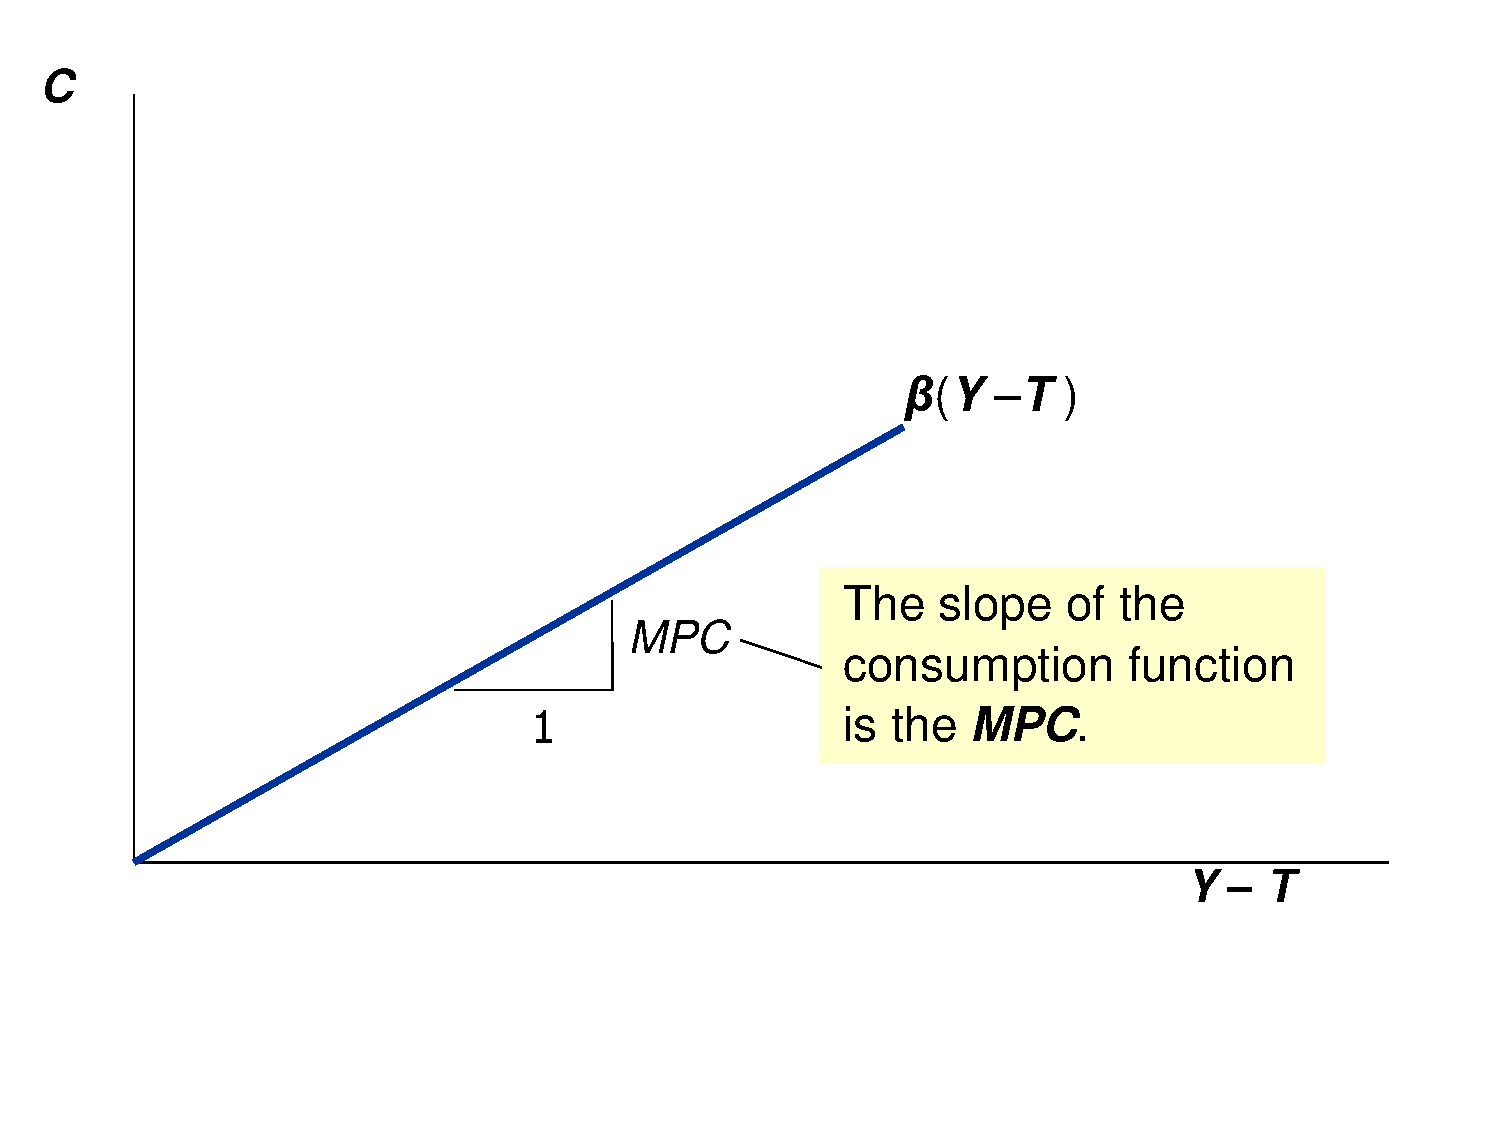
\includegraphics[height=3.1in,width=4.25in]{../figures/mpc.pdf}
\end{center}
\end{frame}

%%%%%%%%%%%%%%%%%%%%%%%%%%%%%%%%%%%%%%%%%%%%%%%%%%%%%%%%%%%%%%%%%%%%%%%%%%%%%%%%%%%%%%%%%%%%%%%%%%
%%%%%%%%%%%%%%%%%%%%%%%%%%%%%%%%%%%%%%%%%%%%%%%%%%%%%%%%%%%%%%%%%%%%%%%%%%%%%%%%%%%%%%%%%%%%%%%%%%

\begin{frame}[t]
\frametitle{Investment}
\begin{itemize}
\item Investment function is: $I = I(r)$
\begin{itemize}
\medskip
\item \small Where $r =$ real interest rate (nominal interest rate adjusted for inflation).
\end{itemize}
\bigskip
\item The real interest rate is,
\begin{itemize}
\medskip
\item \small the cost of borrowing,
\medskip
\item the opportunity cost of using one�s own funds to finance investment spending.
\end{itemize}
\bigskip
\item So $\uparrow r$ implies that $\downarrow I$.
\end{itemize}
\end{frame}


%%%%%%%%%%%%%%%%%%%%%%%%%%%%%%%%%%%%%%%%%%%%%%%%%%%%%%%%%%%%%%%%%%%%%%%%%%%%%%%%%%%%%%%%%%%%%%%%%%
%%%%%%%%%%%%%%%%%%%%%%%%%%%%%%%%%%%%%%%%%%%%%%%%%%%%%%%%%%%%%%%%%%%%%%%%%%%%%%%%%%%%%%%%%%%%%%%%%%
%
%\begin{frame}[t]
%\frametitle{The Real Interest Rate and MPK}
%\begin{itemize}
%\item From profit maximization earlier, real rental rate of capital is
%\begin{eqnarray*}
%\mbox{MPK} = \alpha AK^{\alpha-1}L^{1-\alpha} = R/P, \\
%\\
%\mbox{MPK} = \alpha \frac{Y}{K} = R/P.
%\end{eqnarray*}
%\medskip
%\item I'm asserting this: $R/P =$ r + depreciation
%\bigskip
%\item This implies the real interest rate (r) is connected to the marginal product of capital:\\
%\bigskip
%r = MPK - depreciation
%\end{itemize}
%\end{frame}

%%%%%%%%%%%%%%%%%%%%%%%%%%%%%%%%%%%%%%%%%%%%%%%%%%%%%%%%%%%%%%%%%%%%%%%%%%%%%%%%%%%%%%%%%%%%%%%%%%
%%%%%%%%%%%%%%%%%%%%%%%%%%%%%%%%%%%%%%%%%%%%%%%%%%%%%%%%%%%%%%%%%%%%%%%%%%%%%%%%%%%%%%%%%%%%%%%%%%

\begin{frame}[t]
\frametitle{Investment Function}
\begin{center}
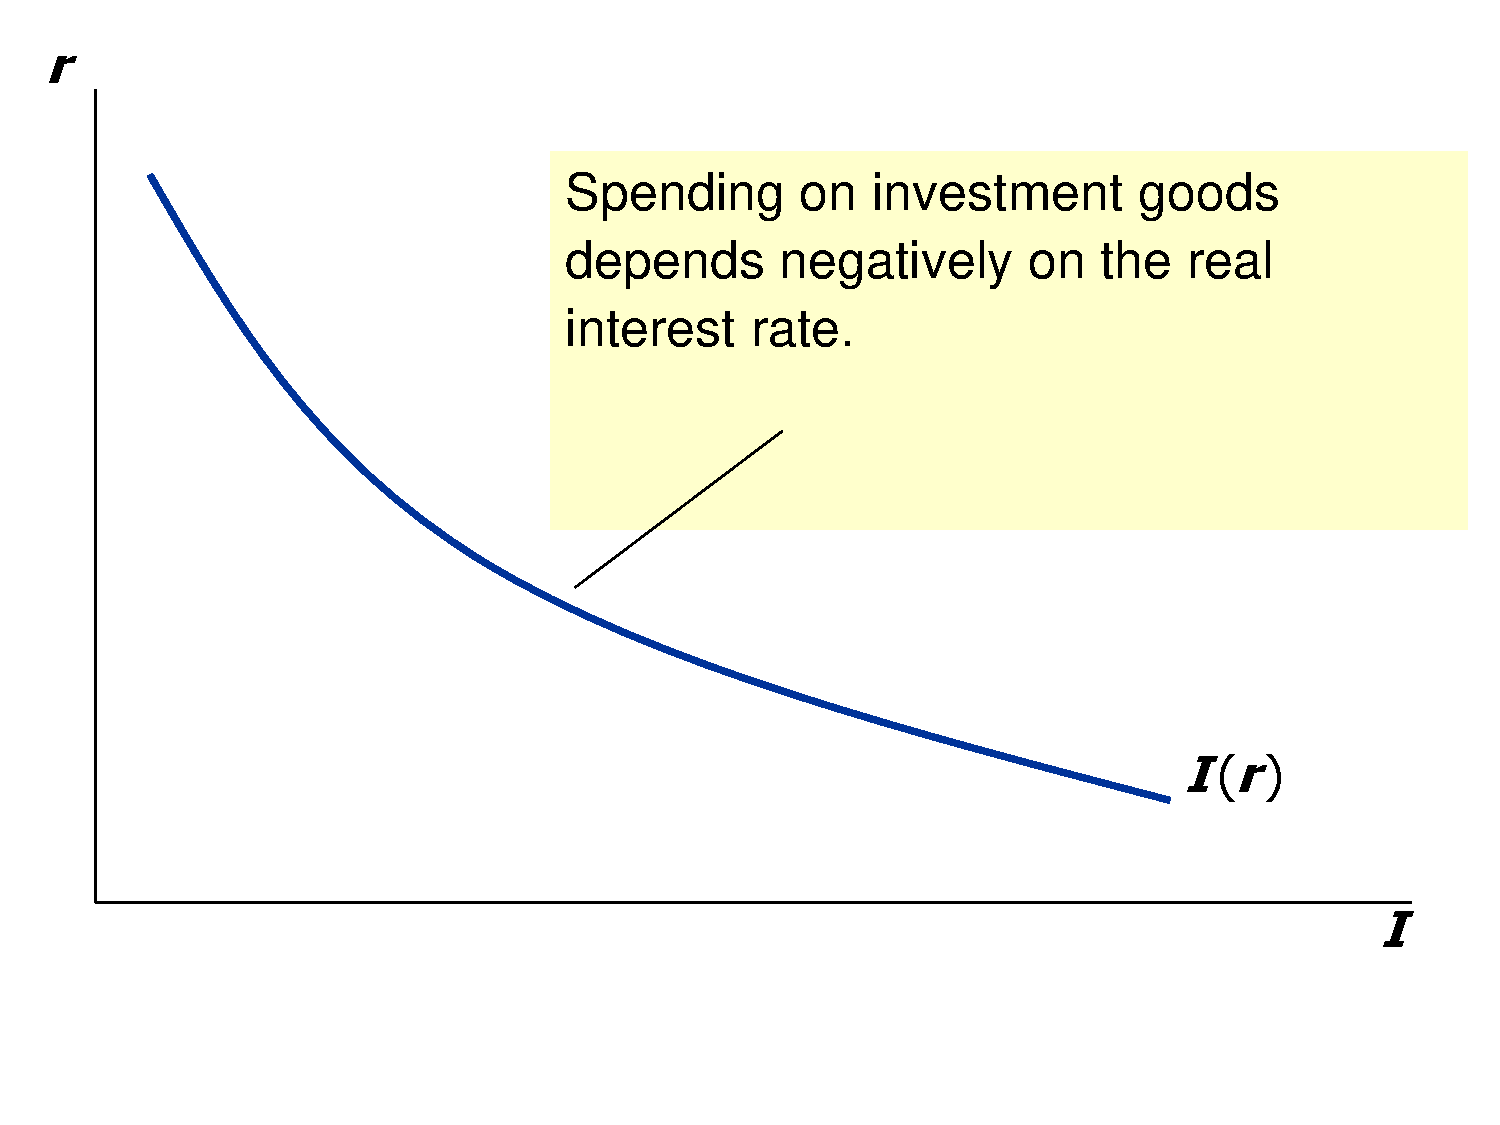
\includegraphics[height=3.1in,width=4.25in]{../figures/investment.pdf}
\end{center}
\end{frame}

%%%%%%%%%%%%%%%%%%%%%%%%%%%%%%%%%%%%%%%%%%%%%%%%%%%%%%%%%%%%%%%%%%%%%%%%%%%%%%%%%%%%%%%%%%%%%%%%%%
%%%%%%%%%%%%%%%%%%%%%%%%%%%%%%%%%%%%%%%%%%%%%%%%%%%%%%%%%%%%%%%%%%%%%%%%%%%%%%%%%%%%%%%%%%%%%%%%%%

\begin{frame}[t]
\frametitle{Government}
\begin{itemize}
\item G  $=$ govt spending on goods and services
\begin{itemize}
\medskip
\item \small G excludes transfer payments (e.g., Social Security benefits, unemployment insurance benefits), just purchases of new goods and services.
\end{itemize}
\bigskip
\item Assume government spending and total taxes are exogenous:
\begin{eqnarray*}
G = \bar G \quad \quad T = \bar T
\end{eqnarray*}
\end{itemize}
\end{frame}

%%%%%%%%%%%%%%%%%%%%%%%%%%%%%%%%%%%%%%%%%%%%%%%%%%%%%%%%%%%%%%%%%%%%%%%%%%%%%%%%%%%%%%%%%%%%%%%%%%
%%%%%%%%%%%%%%%%%%%%%%%%%%%%%%%%%%%%%%%%%%%%%%%%%%%%%%%%%%%%%%%%%%%%%%%%%%%%%%%%%%%%%%%%%%%%%%%%%%

\begin{frame}[t]
\frametitle{Equilibrium \#1: Goods Market}
\begin{itemize}
\item Aggregate Demand:
\begin{eqnarray*}
\underbrace{\beta (\bar Y - \bar T)}_{C} + I(r) + \bar G.
\end{eqnarray*}
\bigskip
\item Aggregate Supply:
\begin{eqnarray*}
\bar Y = \mbox{F}(\bar K, \bar L).
\end{eqnarray*}
\bigskip
\item Equilibrium:
\begin{eqnarray*}
\bar Y = \beta (\bar Y - \bar T) + I(r) + \bar G.
\end{eqnarray*}
\medskip
\item The real interest rate adjusts to equate supply with demand.
\end{itemize}
\end{frame}

%%%%%%%%%%%%%%%%%%%%%%%%%%%%%%%%%%%%%%%%%%%%%%%%%%%%%%%%%%%%%%%%%%%%%%%%%%%%%%%%%%%%%%%%%%%%%%%%%%
%%%%%%%%%%%%%%%%%%%%%%%%%%%%%%%%%%%%%%%%%%%%%%%%%%%%%%%%%%%%%%%%%%%%%%%%%%%%%%%%%%%%%%%%%%%%%%%%%%

\begin{frame}[t]
\frametitle{Equilibrium \#2: Loanable Funds Market}
\begin{itemize}
\item Equilibrium:
\begin{eqnarray*}
\bar Y = \beta (\bar Y - \bar T) + I(r) + \bar G.
\end{eqnarray*}
\item Rearranging
\begin{eqnarray*}
S = \underbrace{\underbrace{\bar Y - \bar T -\beta (\bar Y-\bar T)}_{\small \mbox{Private \ Savings}} \ \ \ \ + \underbrace{\bar T - \bar G}_{\small \mbox{Public\ Savings}} }_{\mbox{National Savings}} = I(r)
\end{eqnarray*}
\medskip
\item The real interest rate adjusts to equate savings with investment!
\begin{itemize}
\medskip
\item This is called ``loanable funds'' market condition. Financial intermediation plays a role here, i.e. connects households who save with firms who investment.
\end{itemize}
\end{itemize}
\end{frame}

%%%%%%%%%%%%%%%%%%%%%%%%%%%%%%%%%%%%%%%%%%%%%%%%%%%%%%%%%%%%%%%%%%%%%%%%%%%%%%%%%%%%%%%%%%%%%%%%%%
%%%%%%%%%%%%%%%%%%%%%%%%%%%%%%%%%%%%%%%%%%%%%%%%%%%%%%%%%%%%%%%%%%%%%%%%%%%%%%%%%%%%%%%%%%%%%%%%%%

\begin{frame}[t]
\frametitle{Supply of Savings}
\begin{center}
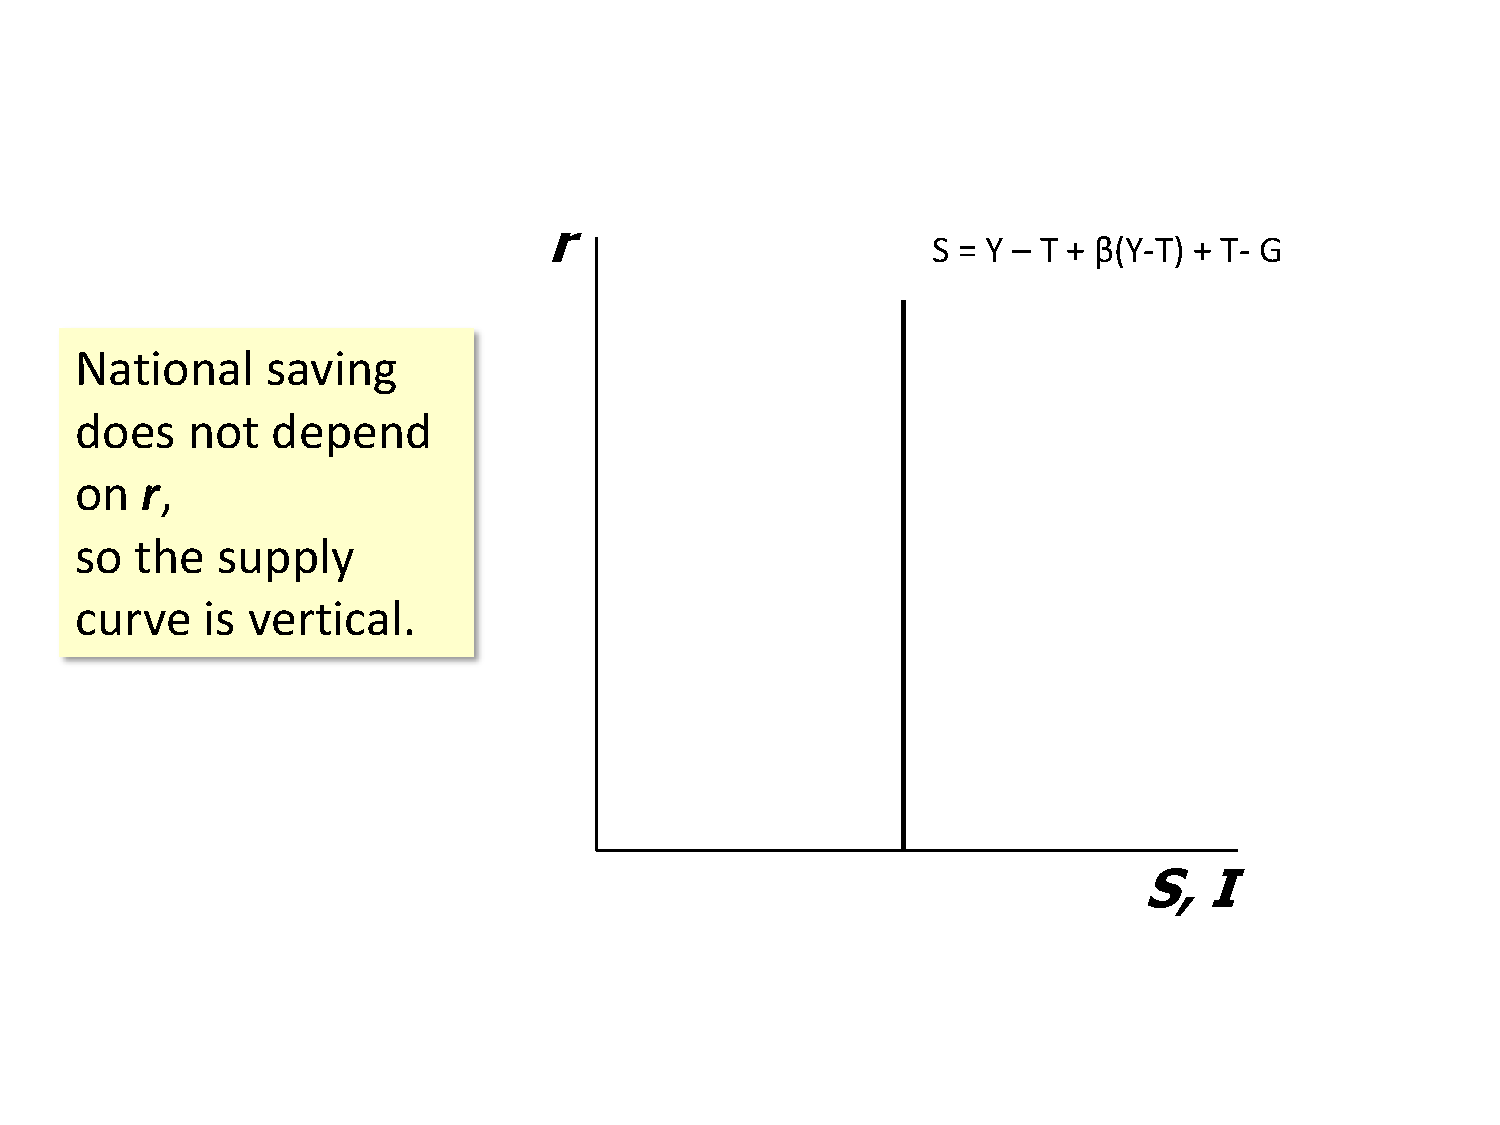
\includegraphics[height=3.1in,width=4.25in]{../figures/savins_funds.pdf}
\end{center}
\end{frame}

%%%%%%%%%%%%%%%%%%%%%%%%%%%%%%%%%%%%%%%%%%%%%%%%%%%%%%%%%%%%%%%%%%%%%%%%%%%%%%%%%%%%%%%%%%%%%%%%%%
%%%%%%%%%%%%%%%%%%%%%%%%%%%%%%%%%%%%%%%%%%%%%%%%%%%%%%%%%%%%%%%%%%%%%%%%%%%%%%%%%%%%%%%%%%%%%%%%%%

\begin{frame}[t]
\frametitle{Demand for Investment and Savings}
\begin{center}
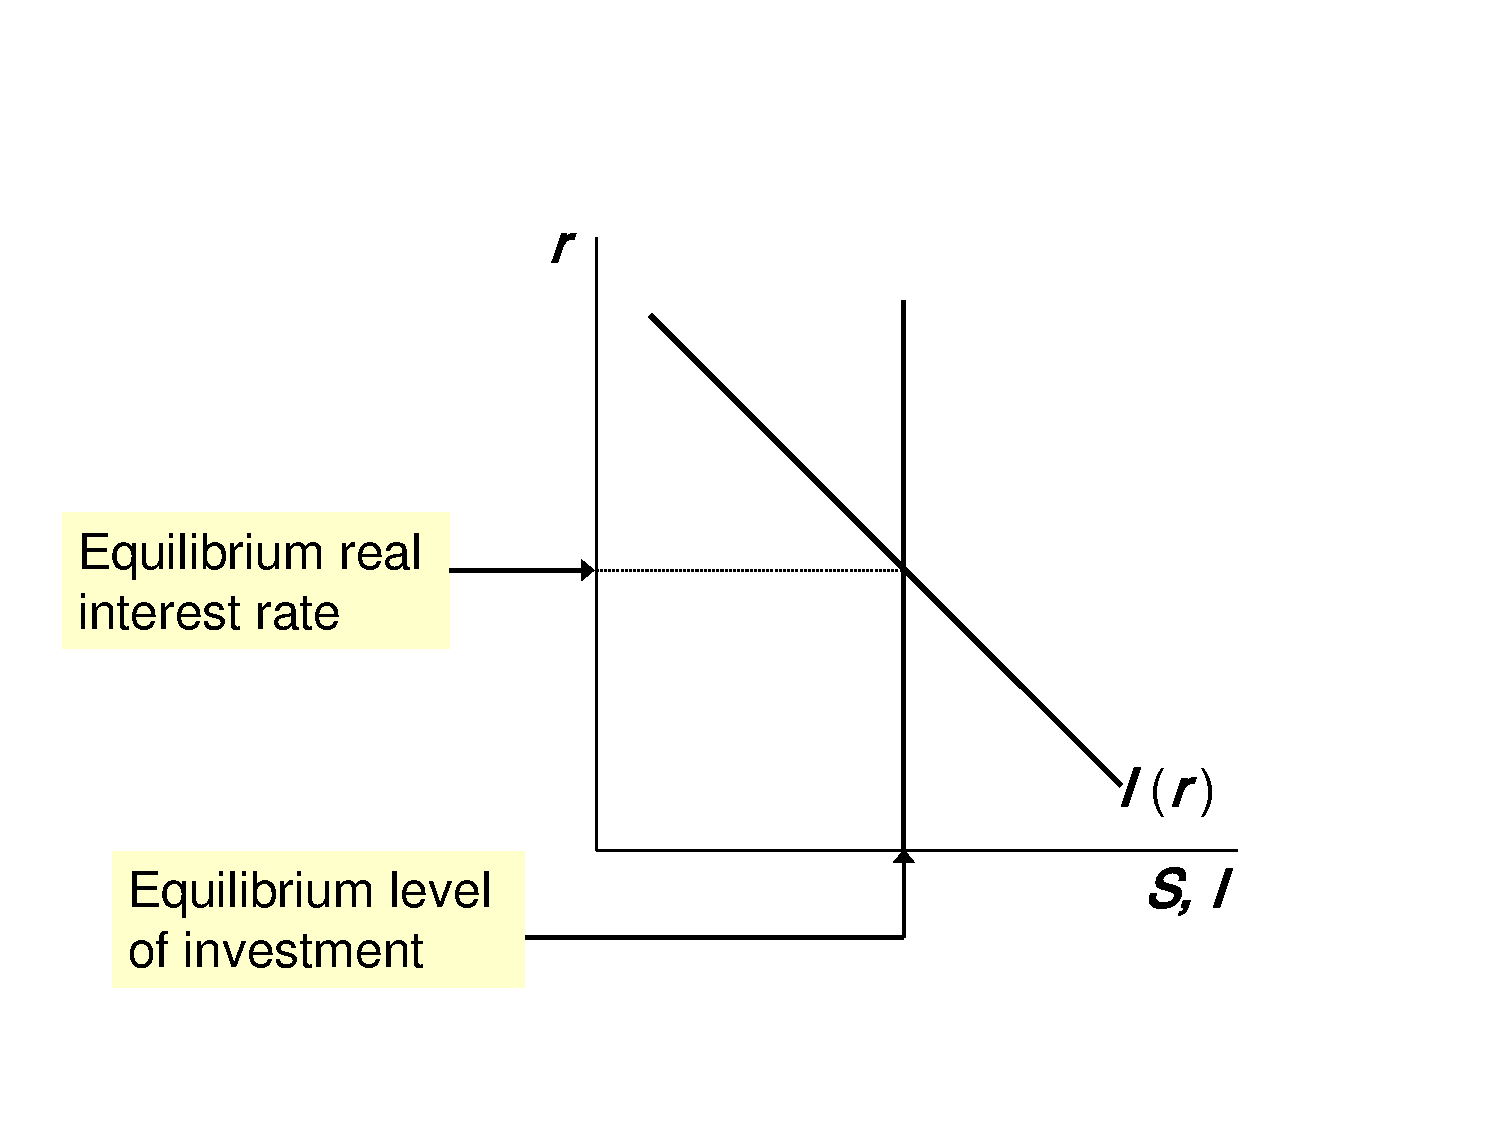
\includegraphics[height=3.1in,width=4.25in]{../figures/loanable_funds.pdf}
\end{center}
\end{frame}

%%%%%%%%%%%%%%%%%%%%%%%%%%%%%%%%%%%%%%%%%%%%%%%%%%%%%%%%%%%%%%%%%%%%%%%%%%%%%%%%%%%%%%%%%%%%%%%%%%
%%%%%%%%%%%%%%%%%%%%%%%%%%%%%%%%%%%%%%%%%%%%%%%%%%%%%%%%%%%%%%%%%%%%%%%%%%%%%%%%%%%%%%%%%%%%%%%%%%

\begin{frame}[t]
\frametitle{Interest Rates and Government Spending}
\begin{itemize}
\item Question:
\begin{itemize}
\medskip
\item Suppose the government starts to spend more on goods and services. For example, military spending in response to a war.
\bigskip
\item What will happen to national savings? Real interest rates?
\bigskip
\item Does it matter if it is deficit neutral. That is higher $G$ is financed through increased taxes?
\end{itemize}
\end{itemize}
\bigskip
\end{frame}

%%%%%%%%%%%%%%%%%%%%%%%%%%%%%%%%%%%%%%%%%%%%%%%%%%%%%%%%%%%%%%%%%%%%%%%%%%%%%%%%%%%%%%%%%%%%%%%%%%
%%%%%%%%%%%%%%%%%%%%%%%%%%%%%%%%%%%%%%%%%%%%%%%%%%%%%%%%%%%%%%%%%%%%%%%%%%%%%%%%%%%%%%%%%%%%%%%%%%

\begin{frame}[t]
\frametitle{Interest Rates and Government Spending}
\begin{center}
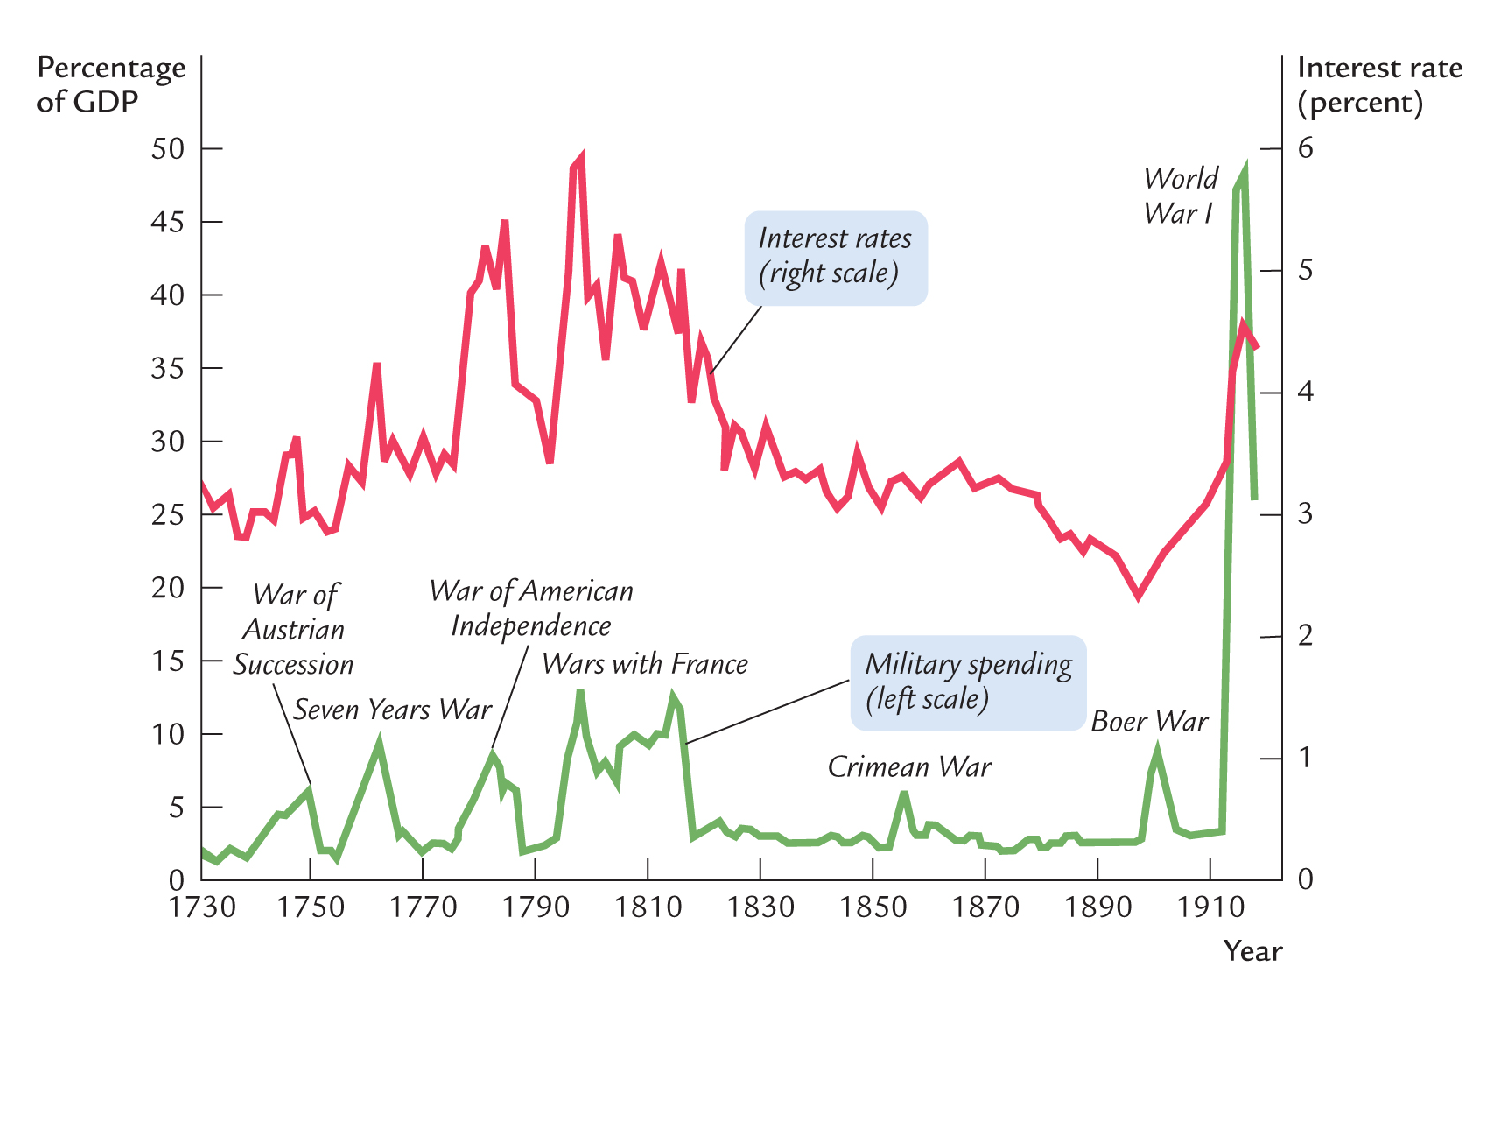
\includegraphics[height=3.1in,width=4.25in]{../figures/war_spending.pdf}
\end{center}
\end{frame}

%%%%%%%%%%%%%%%%%%%%%%%%%%%%%%%%%%%%%%%%%%%%%%%%%%%%%%%%%%%%%%%%%%%%%%%%%%%%%%%%%%%%%%%%%%%%%%%%%%
%%%%%%%%%%%%%%%%%%%%%%%%%%%%%%%%%%%%%%%%%%%%%%%%%%%%%%%%%%%%%%%%%%%%%%%%%%%%%%%%%%%%%%%%%%%%%%%%%%

\begin{frame}[t]
\frametitle{Changes in Investment Demand}
\begin{itemize}
\item Things that shift (increase) the investment curve: Anything that increases the marginal product of capital.
\begin{itemize}
\medskip
\item More labor? Yes.\\
\medskip
Why? Need more capital to go along with labor, thus the demand for investment increases.
\bigskip
\item Better Technology ($A$)? Yes.\\
\medskip
Why? Capital is now more productive, thus the demand for instatement increases.
\end{itemize}
\medskip
\item At home: Holding savings fixed, how will these scenarios affect $r$?
\end{itemize}
\bigskip
\end{frame}

%%%%%%%%%%%%%%%%%%%%%%%%%%%%%%%%%%%%%%%%%%%%%%%%%%%%%%%%%%%%%%%%%%%%%%%%%%%%%%%%%%%%%%%%%%%%%%%%%%
%%%%%%%%%%%%%%%%%%%%%%%%%%%%%%%%%%%%%%%%%%%%%%%%%%%%%%%%%%%%%%%%%%%%%%%%%%%%%%%%%%%%%%%%%%%%%%%%%%

\begin{frame}[t]
\frametitle{Chapter 3 Takeaways}
\begin{itemize}
\item Total output/value added is determined by:
\begin{itemize}
\medskip
\item The economy�s quantities of capital and labor,
\medskip
\item The level of technology (total factor productivity).
\end{itemize}
\bigskip
\item Income payments to labor and capital are determined by
\begin{itemize}
\medskip
\item The economy�s quantities of capital and labor
\medskip
\item Competitive firms hire each factor until its marginal product equals its price.
\end{itemize}
\bigskip
\item Allocation of output to (C, I, G) determined by
\begin{itemize}
\medskip
\item The real interest rate adjusts to equate the demand and supply of savings/investment.
\end{itemize}
\end{itemize}
\end{frame}

\end{document} 